\documentclass[11pt]{article}
\usepackage{amsthm}
\usepackage{amssymb}
\usepackage{enumitem}
\usepackage{amsmath, physics}
\usepackage{bm}
\usepackage{adjustbox}
\usepackage{mathrsfs}
\usepackage{graphicx}
\usepackage{siunitx}
\usepackage[mathscr]{euscript}

\title{\textbf{Solved selected problems of Modern Physics for Scientists and Engineers - John Taylor}}
\author{Franco Zacco}
\date{}

\addtolength{\topmargin}{-3cm}
\addtolength{\textheight}{3cm}

\newcommand{\N}{\mathbb{N}}
\newcommand{\Z}{\mathbb{Z}}
\newcommand{\Q}{\mathbb{Q}}
\newcommand{\R}{\mathbb{R}}
\newcommand{\diam}{\text{diam}}
\newcommand{\cl}{\text{cl}}
\newcommand{\bdry}{\text{bdry}}
\newcommand{\inter}{\text{int}}
\newcommand{\hatx}{\bm{\hat{x}}}
\newcommand{\haty}{\bm{\hat{y}}}
\newcommand{\hatz}{\bm{\hat{z}}}
\newcommand{\hatrho}{\bm{\hat{\rho}}}
\newcommand{\hatphi}{\bm{\hat{\phi}}}
\newcommand{\hatr}{\bm{\hat{r}}}
\newcommand{\hattheta}{\bm{\hat{\theta}}}
\newcommand{\sci}[1]{\times 10^{#1}}
\newcommand{\expect}[1]{\left\langle {#1} \right\rangle}

\theoremstyle{definition}
\newtheorem*{solution*}{Solution}
\renewcommand*{\proofname}{\bf{Solution}}

\begin{document}
\maketitle
\thispagestyle{empty}

\section*{Chapter 9 - Electron Spin}

\begin{proof}{\textbf{9.2}}
\begin{itemize}
\item [\textbf{(a)}] For a particle with $s = 3/2$ there are four possible
values of $S_z$ and they are
\begin{align*}
    \frac{3}{2}\hbar,\quad\frac{1}{2}\hbar,\quad-\frac{1}{2}\hbar,
    \quad-\frac{3}{2}\hbar
\end{align*}
\item [\textbf{(b)}] Below we show the requested vector model diagram
\begin{center}
    % 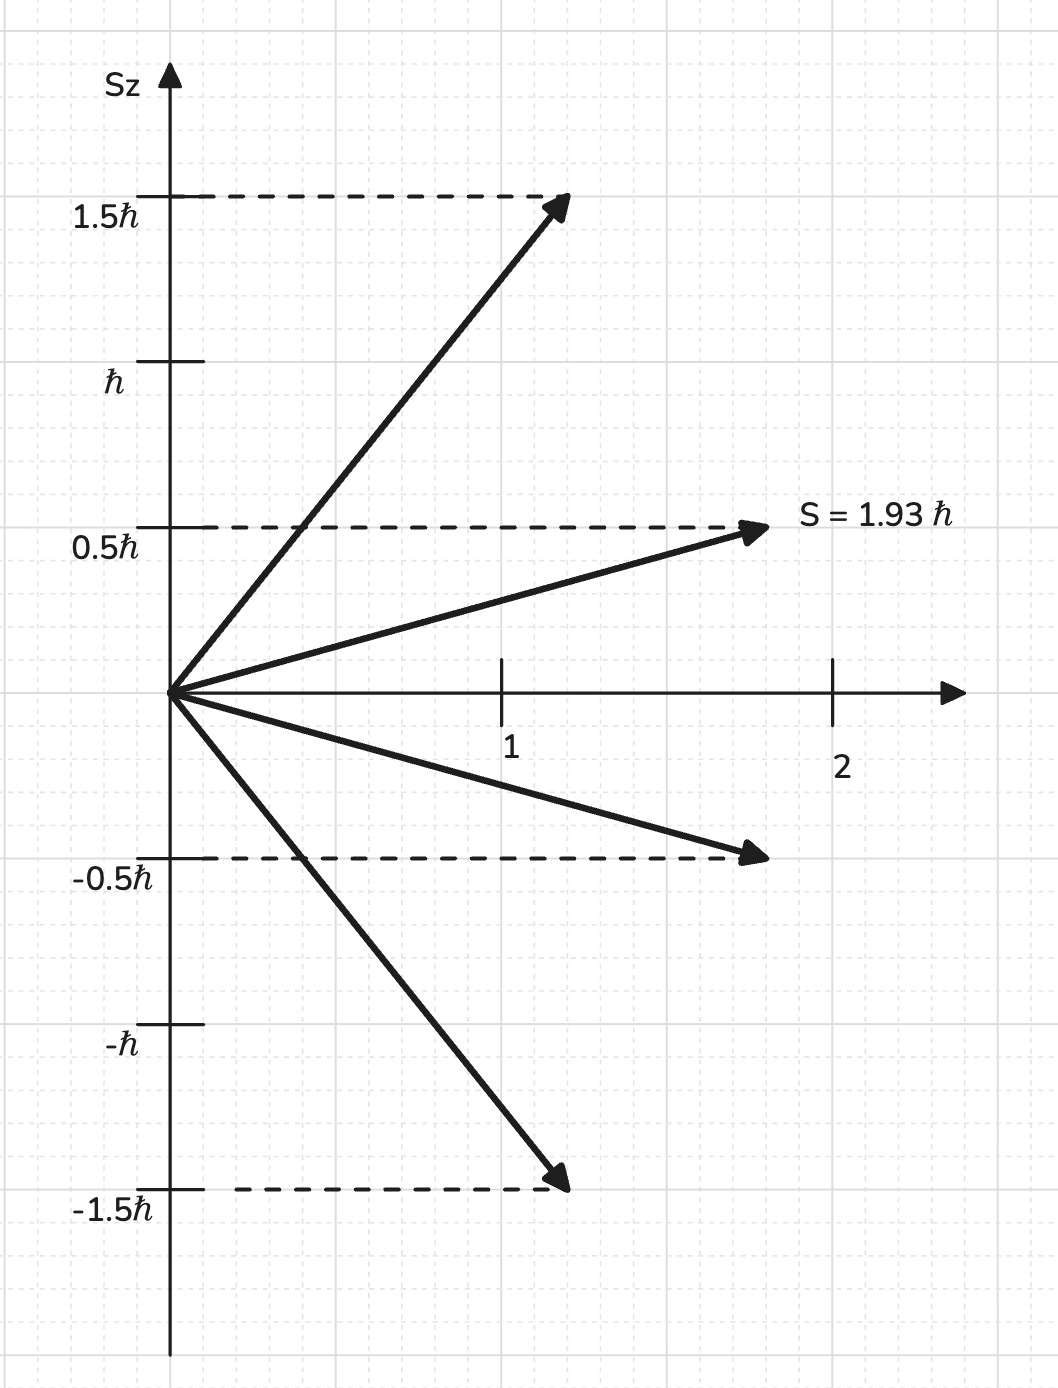
\includegraphics[scale=0.35]{ch9-9.2.png}
\end{center}
\item [\textbf{(c)}] The minimum possible angle between $\bm{S}$ and the
$z$-axis is given by
\begin{align*}
    \cos\theta = \frac{3\hbar/2}{\sqrt{15}\hbar/2} = \frac{3}{\sqrt{15}}
\end{align*}
Which implies that $\theta \approx 39.23^\circ$
\end{itemize}
\end{proof}

\cleardoublepage
\begin{proof}{\textbf{9.3}}
\begin{itemize}
\item [\textbf{(a)}] For a particle with $s = 1$ there are three possible
values of $S_z$ and they are
\begin{align*}
    \hbar,\quad 0,\quad-\hbar
\end{align*}
\item [\textbf{(b)}] Below we show the requested vector model diagram
\begin{center}
    % 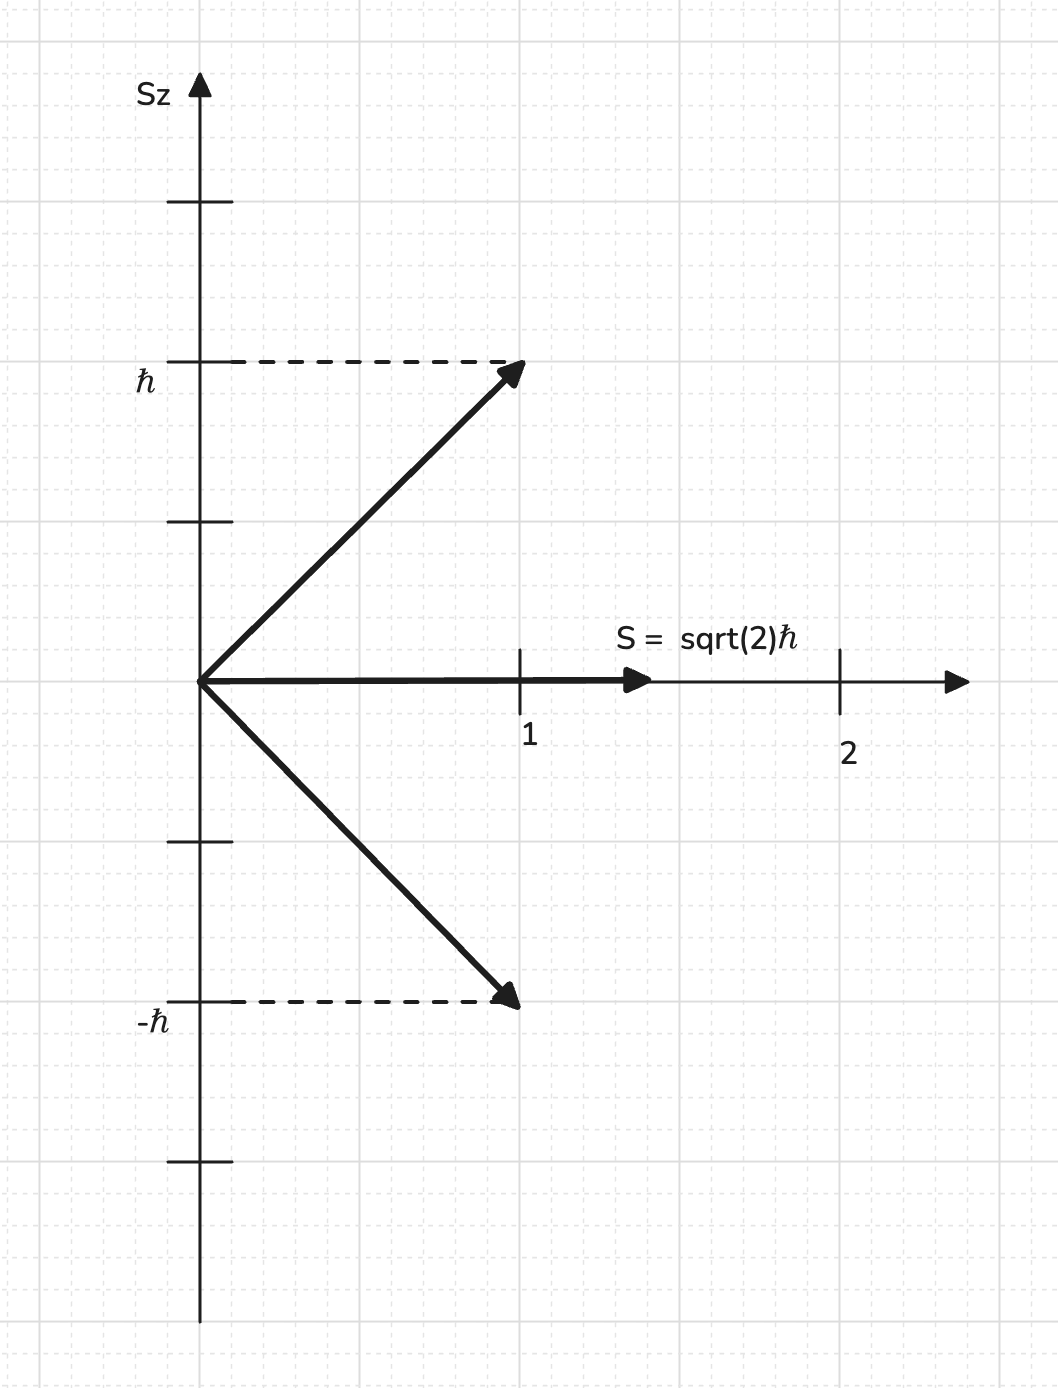
\includegraphics[scale=0.35]{ch9-9.3.png}
\end{center}
\item [\textbf{(c)}] The minimum possible angle between $\bm{S}$ and the
$z$-axis is given by
\begin{align*}
    \cos\theta = \frac{\hbar}{\hbar} = 1
\end{align*}
Which implies that $\theta = 0^\circ$
\end{itemize}
\end{proof}

\cleardoublepage
\begin{proof}{\textbf{9.6}}
\begin{itemize}
\item [\textbf{(a)}] For an $s$ electron we have that
$L = \sqrt{0(0 + 1)}\hbar = 0$ so
\begin{align*}
    \frac{S}{L} = \frac{\sqrt{3}\hbar/2}{0} = \infty
\end{align*}
\item [\textbf{(b)}] For a $p$ electron we have that
$L = \sqrt{1(1 + 1)}\hbar = \sqrt{2}\hbar$ so
\begin{align*}
    \frac{S}{L} = \frac{\sqrt{3}\hbar/2}{\sqrt{2}\hbar}
    = \frac{\sqrt{6}}{4} = 0.612
\end{align*}
\item [\textbf{(c)}] For a $d$ electron we have that
$L = \sqrt{2(2 + 1)}\hbar = \sqrt{6}\hbar$ so
\begin{align*}
    \frac{S}{L} = \frac{\sqrt{3}\hbar/2}{\sqrt{6}\hbar}
    = \frac{\sqrt{2}}{4} = 0.353
\end{align*}
\item [\textbf{(d)}] For an $f$ electron we have that
$L = \sqrt{3(3 + 1)}\hbar = \sqrt{12}\hbar$ so
\begin{align*}
    \frac{S}{L} = \frac{\sqrt{3}\hbar/2}{\sqrt{12}\hbar}
    = \frac{1}{4} = 0.25
\end{align*}
\end{itemize}
\end{proof}

\cleardoublepage
\begin{proof}{\textbf{9.8}}
If we consider the electron to be a spinning ball of matter,
considering the velocity at the equator $v$ and the upper bound of
the radius of the electron $r$, then the angular momentum is
\begin{align*}
    L = m_e vr
\end{align*}
Since we know that $L = \sqrt{3}\hbar/2$ then we can determine the velocity of
rotation to be
\begin{align*}
    v = \frac{L}{m_e r} = \frac{\sqrt{3}\hbar/2}{9.109\sci{-31}\cdot 10^{-18}}
    = 1.003 \sci{14}~m/s
\end{align*}
Then we see that
\begin{align*}
    \frac{v}{c} = \frac{1.003 \sci{14}}{2.998\sci{8}} = 334556.37
\end{align*}
Implying that the electron is spinning $334556.37$ times faster than the speed
of light, which is not possible according to relativity.
\end{proof}

\cleardoublepage
\begin{proof}{\textbf{9.9}}
Let a current of $0.4~A$ flow around a single circular loop of radius $1~cm$.
\begin{itemize}
\item [\textbf{(a)}] The magnitude of the magnetic moment, $\mu$, is
\begin{align*}
    \mu = iA = i \pi r^2 = 1.256~A cm^2 = 0.0001256~A m^2
\end{align*}
\item [\textbf{(b)}] Let $\bm\mu$ be perpendicular to $\bm{B}$ where $B = 1.5~T$
then the torque on the loop has a magnitude
\begin{align*}
    \Gamma = \mu B\sin \theta = \mu B = 0.0001256~A m^2 \cdot 1.5~T
    = 0.0001883~Nm
\end{align*}
\item [\textbf{(c)}] When $\bm{\mu}$ is parallel to $\bm{B}$ the energy is
\begin{align*}
    U_p = -\mu B\cos(0) = -\mu B = -0.0001883~J
\end{align*}
And when they are antiparallel the energy is
\begin{align*}
    U_{ap} = -\mu B\cos(\pi) = \mu B = 0.0001883~J
\end{align*}
So the difference in energy is
\begin{align*}
    |U_p - U_{ap}| = |-0.0001883~J - (0.0001883~J)| = 0.0003766~J
\end{align*}
\end{itemize}
\end{proof}

\cleardoublepage
\begin{proof}{\textbf{9.11}}
Given that a typical atomic magnetic moment is of order $10^{-23}~Am^2$
assuming a single circular loop of radius $0.1~nm$ then $i$ is
\begin{align*}
    i = \frac{\mu}{A} = \frac{\mu}{\pi r^2}
    = \frac{10^{-23}}{\pi(0.1\sci{-9})^2}
    = 0.000318~A
\end{align*}
\end{proof}
\begin{proof}{\textbf{9.12}}
The magnetic energy due to the orbital magnetic moment in the direction of the
$z$-axis is
\begin{align*}
    U_z = -\mu_z B = - \frac{e}{2m_e}\hbar \cdot B
\end{align*}
Then for a $B = 10~T$ we have that
\begin{align*}
    U_z &= - \frac{1.602\sci{-19}~C}{2\cdot 9.109\sci{-31}~kg}
    \cdot 1.055 \sci{-34}~\frac{m^2kg}{s}\cdot 10~T\\
    &= -9.277\sci{-23}~J = -5.79\sci{-4}~eV
\end{align*}
\end{proof}

\cleardoublepage
\begin{proof}{\textbf{9.15}}
Let a helium atom in an energy level with one electron occupying an $s$ state
$(l = 0)$ and the other in an $f$ state $(l = 3)$.
\\
The two electron spins are antiparallel so that the spin magnetic moments cancel.
The atom is placed in a magnetic field $B = 0.8~T$.
\begin{itemize}
\item [\textbf{(a)}] Below, on the right, we show a sketch of the resulting
splitting of the original energy level.
\begin{center}
    % 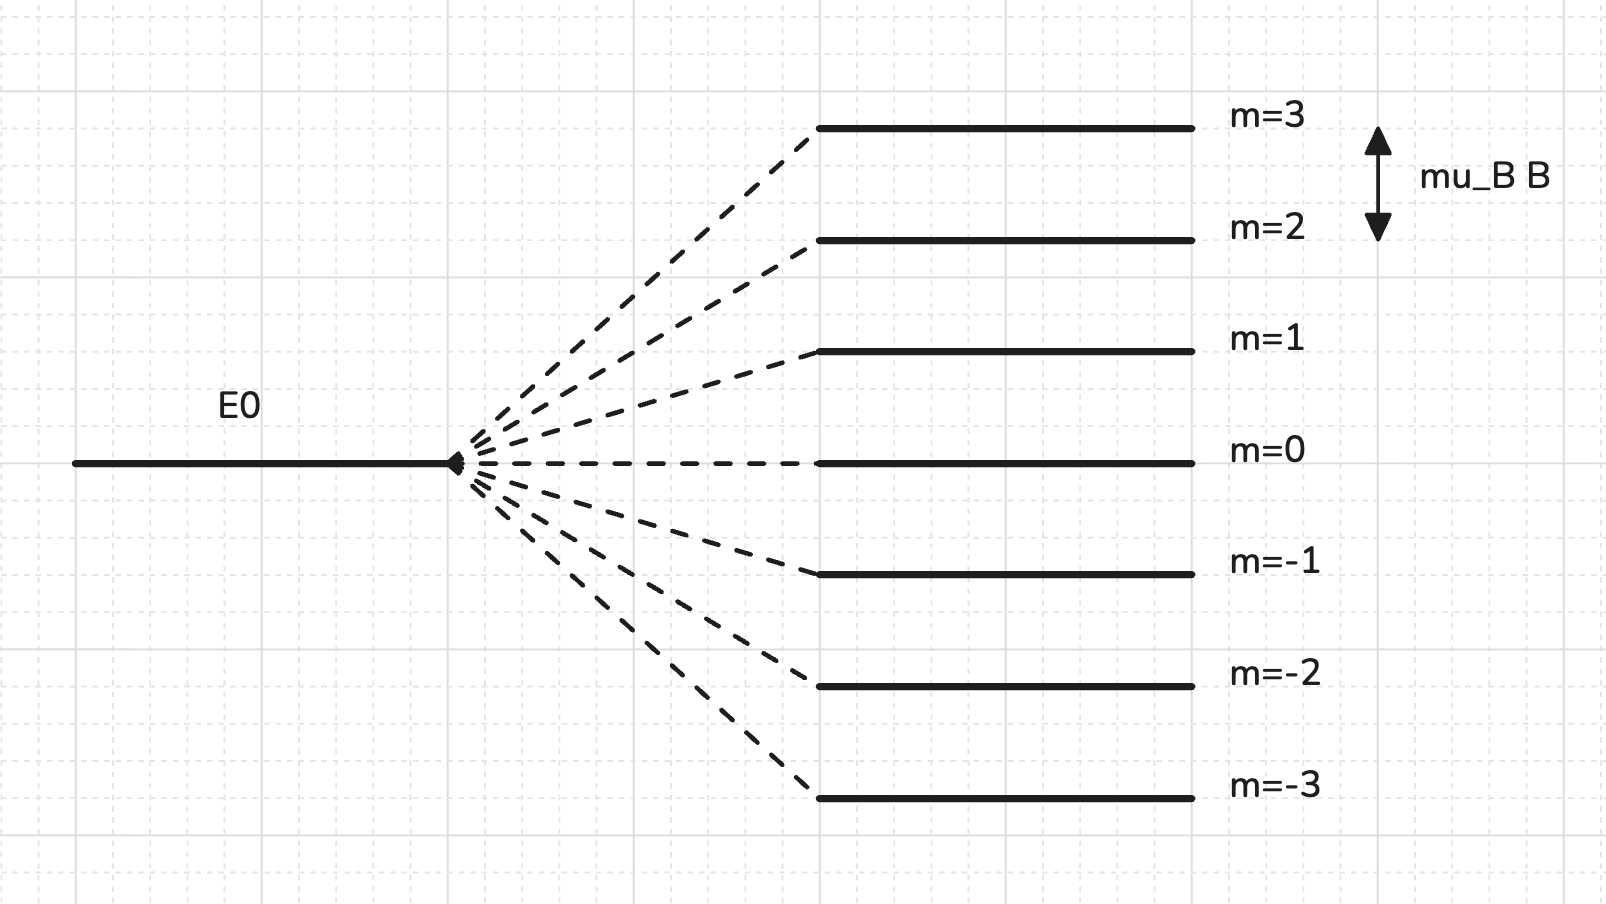
\includegraphics[scale=0.3]{ch9-9.15.png}
\end{center}
\item [\textbf{(b)}] The energy difference between adjacent levels of the
resulting multiplet is given by
\begin{align*}
    \mu_B B = 5.79\sci{-5}~eV/T \cdot 0.8~T = 4.63\sci{-5}~eV
\end{align*}
Assuming the magnetic field is in the direction of $L_z$.
\end{itemize}
\end{proof}

\cleardoublepage
\begin{proof}{\textbf{9.16}}
\begin{itemize}
\item [\textbf{(a)}] The $B$ field will not affect the $1s$ state since $l = 0$
for this case and hence the only value $m$ can take is $m = 0$.
\\
For the state $2p$ we have that $l = 1$ so $m$ can take the values $-1, 0 $ and
$1$. Then the magnetic field $B$ will split this energy level into three
different ones.
\begin{center}
    % 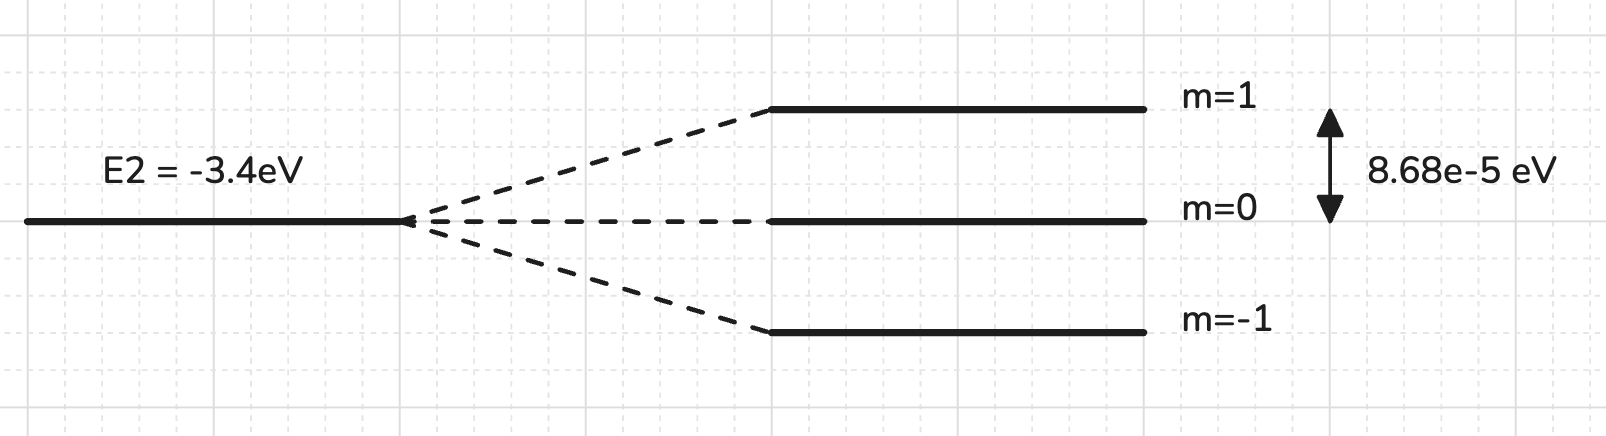
\includegraphics[scale=0.3]{ch9-9.16.png}
\end{center}
\item [\textbf{(b)}] When $B$ is switched on there are three spectral lines due
to the split of the energy level $E_2$ associated to the state $2p$.
\item [\textbf{(c)}] We know that the energy difference between the state $1s$
and $2p$ is
\begin{align*}
    E_2 - E_1  = -3.4eV + 13.6 eV = 10.2~eV
\end{align*}
So the frequency of the photon emited when the electon drops from the state $2p$
to $1s$ is
\begin{align*}
    f_0 = \frac{E_2 - E_1}{h} = \frac{10.2~eV}{4.135\sci{-15}~eVs}
    = 2.466 \sci{15}~Hz
\end{align*}
And the frequency difference due to the magnetic field, $\Delta f$, is
\begin{align*}
    \Delta f = \frac{\mu_B B}{h}
    = \frac{5.79\sci{-5}~eV/T \cdot 1.5~T}{4.135\sci{-15}~eVs}
    = 2.1\sci{10}~Hz
\end{align*}
Then the fractional separation between adjacent lines is
\begin{align*}
    \frac{\Delta f}{f_0} = \frac{2.1\sci{10}~Hz}{2.466 \sci{15}~Hz}
    = 8.515 \sci{-6}
\end{align*}
\end{itemize}
\end{proof}

\cleardoublepage
\begin{proof}{\textbf{9.17}}
\begin{itemize}
\item [\textbf{(a)}] In the top part of the sketch we show the split of the 
electron's energy in the $d$ state and in the lower part the split of the
electron's energy in the $p$ state due to the magnetic field.
\begin{center}
    \includegraphics*[scale=0.35]{ch9-9.17.png}
\end{center}
\item [\textbf{(b)}]
The photon energy is determined by
\begin{align*}
    E_i - E_f &= (E_d + m_i \mu_B B) - (E_p + m_f \mu_B B)\\
    &= E_d - E_p + \mu_B B(m_i  - m_f)
\end{align*}
So the number of possible photon energies is given by the number of different
$(m_i  - m_f)$ we can have.
\\
If $m_i = 2$ the different differences we can have are
\begin{align*}
    2 - 1 &= 1\\
    2 - 0 &= 2 \\
    2 - (-1) &= 3
\end{align*}
If $m_i = 1$
\begin{align*}
    1 - 1 &= 0 \\
    1 - 0 &= 1 \text{ (repeated)}\\
    1 - (-1) &= 2 \text{ (repeated)}
\end{align*}
If $m_i = 0$
\begin{align*}
    0 - 1 &= -1 \\
    0 - 0 &= 0 \text{ (repeated)}\\
    0 - (-1) &= 2 \text{ (repeated)}
\end{align*}
If $m_i = -1$
\begin{align*}
    -1 - 1 &= -2 \\
    -1 - 0 &= -1 \text{ (repeated)}\\
    -1 - (-1) &= 0 \text{ (repeated)}
\end{align*}
And if $m_i = -2$
\begin{align*}
    -2 - 1 &= -3 \\
    -2 - 0 &= -2 \text{ (repeated)}\\
    -2 - (-1) &= -1 \text{ (repeated)}
\end{align*}
Therefore the possible differences are
\begin{align*}
    (m_i - m_f) \in \{-3, -2, -1, 0, 1, 2, 3\}
\end{align*}
So there are 7 possible photon energies.
\end{itemize}
\item[\textbf{(c)}] Because the difference $(m_i -m_f)$ can only take the values
$-1, 0$ or $1$ then because of what we saw in part (b) we get that there are
only three possible photon energies.
\end{proof}

\cleardoublepage
\begin{proof}{\textbf{9.18}}
Let $\bm{\mu} = -e(\bm{L} + 2\bm{S})/2m_e$ be the electron's total magnetic
moment.
\begin{itemize}
\item [\textbf{(a)}] If $l = 0$ then we get that $\bm{L} = 0$ and hence the
total magnetic moment of the electron becomes 
\begin{align*}
    \bm{\mu} = -\frac{e}{m_e}\bm{S}
\end{align*}
So the total magnetic moment is reduced to the spin magnetic moment of the 
electron.
\\
Since the component $S_z$ is given by $S_z = m_s \hbar$ and $m_s$ can be $1/2$
or $-1/2$ for the electron then $\mu_z$ can have two values
\begin{align*}
    \mu_z = -\frac{e}{m_e}S_z = \begin{cases}
        -\frac{e\hbar}{2m_e} \quad &m_s = \frac{1}{2}\\[7pt]
        +\frac{e\hbar}{2m_e} \quad &m_s = -\frac{1}{2}
    \end{cases}
\end{align*}
\item [\textbf{(b)}] A hypothetical spinless electron with $l = 1$ will have
a magnetic moment component $\mu_z$ given by
\begin{align*}
    \mu_z = -\frac{e}{2m_e}L_z = -\frac{e}{2m_e}m \hbar
\end{align*}
Where $m = -1, 0, 1$ hence
\begin{align*}
    \mu_z =  -\frac{e}{2m_e}m \hbar = \begin{cases}
        -\frac{e\hbar}{2m_e} &\quad m = 1\\[7pt]
        0 &\quad m = 0\\[7pt]
        +\frac{e\hbar}{2m_e} &\quad m = -1
    \end{cases}
\end{align*}
So compared to part (a) they would have the same magnetic moment component
$\mu_z$.

\end{itemize}
\end{proof}

\cleardoublepage
\begin{proof}{\textbf{9.19}}
Let a hydrogen atom on its ground level placed in a magnetic field of $0.7~T$
along the $z$ axis.
\begin{itemize}
\item [\textbf{(a)}] The energy difference between the spin-up and spin-down
states is given by
\begin{align*}
    \Delta E = 2\mu_B B = 2\cdot 5.79\sci{-5} \cdot 0.7 = 8.106\sci{-5}~eV
\end{align*}
\item [\textbf{(b)}] To excite the atom from the lower to the upper state we
need to send a photon with an energy of $8.106\sci{-5}~eV$ since that's the
energy sparation between the levels. Hence it would need to have a wavelenght
givne by
\begin{align*}
    \lambda = \frac{hc}{\Delta E}
    = \frac{1240~eV\cdot nm}{8.106\sci{-5}~eV}
    = 15297310.63~nm = 1.529~cm
\end{align*}
This radiation falls under the microwave radiation.
\end{itemize}
\end{proof}

\cleardoublepage
\begin{proof}{\textbf{9.20}}
Let us consider a hydrogen atom in the 3d state with $L_z = 2\hbar$ and
$S_z = \frac{1}{2}\hbar$. If we place it in a magnetic field $B = 0.6~T$ along
the $z$ axis its energy will change by
\begin{align*}
    \Delta E &= -\bm{\mu}_{tot}\cdot \bm{B}
    = -\frac{e}{2m_e}(\bm{L} + 2\bm{S})\cdot \bm{B}
    = -\frac{e}{2m_e}(L_z + 2S_z) B
\end{align*}
Hence
\begin{align*}
    \Delta E
    &= -\frac{e}{2m_e}(2\hbar + \hbar) \cdot 0.6\\
    &= -\frac{e\hbar}{2m_e}\cdot 1.8\\
    &= -\mu_B\cdot 1.8\\
    &= -5.79\sci{-5} \cdot 1.8\\
    &= -1.0422\sci{-4}~eV
\end{align*}
\end{proof}

\cleardoublepage
\begin{proof}{\textbf{9.21}}
\begin{itemize}
\item[\textbf{(a)}] We know that the $B$ field at the center of a circular
current loop, $i$, of radius $r$ is known to be
\begin{align*}
    B = \frac{\mu_0 i}{2r}
\end{align*}
Since the current produced by the orbiting proton is
\begin{align*}
    i = \frac{ev}{2\pi r}
\end{align*}
Then 
\begin{align*}
    B = \frac{\mu_0 ev}{4\pi r^2}
\end{align*}
Multiplying and dividing the expression by $m_e r$ where $m_e$ is the mass
of the electron, we get that
\begin{align*}
    B = \frac{\mu_0 e m_e v r}{4\pi m_e r^3}
    = \frac{\mu_0}{4\pi} \frac{e L}{m_e r^3}
\end{align*}
Where we used that $L = m_e vr$ is the electron's orbital angular momentum.

\item[\textbf{(b)}] Let $L = 2\hbar$ and $r = 4a_B$ then $B$ is given by
\begin{align*}
    B &= \frac{\mu_0}{128\pi} \frac{e \hbar}{m_e a_B^3}\\
    &= \frac{4\pi \sci{-7}~Tm/A}{128\pi}
    \frac{1.602 \sci{-19}~C\cdot 1.054\sci{-34}~Js}
    {9.109\sci{-31}~kg \cdot (5.29\sci{-11}~m)^3}\\
    &= 0.39 ~T
\end{align*}
Hence, the separation of the two $2p$ levels is
\begin{align*}
    2\mu_B B = 2 \cdot 5.79\sci{-5}~eV/T \cdot 0.39~T = 4.51\sci{-5}~eV 
\end{align*}
\end{itemize}
\end{proof}

\cleardoublepage
\begin{proof}{\textbf{9.22}}
\begin{itemize}
\item [\textbf{(a)}] The separation of the two $2p$ levels $\Delta E_{FS}$ 
can be written as
\begin{align*}
    \Delta E_{FS} &= 2\mu_B B\\
    &= 2\frac{e\hbar}{2m_e}\frac{\mu_0}{4\pi} \frac{2 e \hbar}{64 m_e a_B^3}\\
    &= 2\frac{e\hbar}{2m_e}\frac{\mu_0\varepsilon_0}{4\pi\varepsilon_0}
    \frac{2 e \hbar (ke^2 m_e)^3}{64 m_e (\hbar^2)^3}\\
    &= \frac{e\hbar}{m_e}\frac{k}{c^2}
    \frac{e \hbar (ke^2 m_e)^3}{32 m_e \hbar^6}\\
    &=\frac{\hbar^2 (ke^2)^4 m_e^3}{32 m_e^2 \hbar^6c^2}\\
    &=\frac{m_e(ke^2)^4}{32 \hbar^4c^2}
\end{align*}
Where we replaced the values of $a_B$ and $\mu_B$.

\item [\textbf{(b)}] We know that
\begin{align*}
    E_R &= \frac{m_e (ke^2)^2}{2\hbar^2}
\end{align*}
Then we can write $\Delta E_{FS}$ as
\begin{align*}
    \Delta E_{FS} &=\frac{m_e(ke^2)^2}{2 \hbar^2}\frac{(ke^2)^2}{16\hbar^2c^2}
    = E_R\frac{(ke^2)^2}{16\hbar^2c^2}
\end{align*}
Defining $\alpha = ke^2/\hbar c$, we see that
\begin{align*}
    \Delta E_{FS} = \frac{\alpha^2E_R}{16}
\end{align*}

\item [\textbf{(c)}] We see that
\begin{align*}
    \alpha = \frac{ke^2}{\hbar c}
    = \frac{8.98\sci{9}\cdot (1.602\sci{-19})^2}{1.054\sci{-34}\cdot 2.9979\sci{8}}
    = 0.007299 \approx \frac{1}{137}
\end{align*}
\end{itemize}
\end{proof}

\cleardoublepage
\begin{proof}{\textbf{9.23}}
\begin{itemize}
\item [\textbf{(a)}] The relativistic kinetic enery expression for the
electron is given by
\begin{align*}
    K = mc^2\bigg(\frac{1}{\sqrt{1 - v^2/c^2}} - 1\bigg)
\end{align*}
Applying the binomial series we get that
\begin{align*}
    K &= mc^2\bigg[\bigg(1 + \frac{1}{2}\frac{v^2}{c^2}
    + \frac{-1/2(-1/2 - 1)}{2}\frac{v^4}{c^4}\bigg) - 1\bigg]\\
    &= mc^2\bigg(
    \frac{1}{2}\frac{v^2}{c^2}
    + \frac{3/4}{2}\frac{v^4}{c^4}\bigg)\\
    &= \frac{1}{2}mv^2
    + \frac{3}{8}\frac{mv^4}{c^2}
\end{align*}
\item [\textbf{(b)}] Replacing $v = \alpha c$, the relativistic correction
gives us
\begin{align*}
    \Delta E_{rel} &= \frac{3}{8}\frac{mv^4}{c^2}
    = \frac{3}{8}\frac{m\alpha^4 c^4}{c^2}
    = \frac{3}{8}\alpha^2\frac{m(ke^2)^2 c^2}{\hbar^2 c^2}
    = \frac{3}{4}\alpha^2\frac{m(ke^2)^2}{2\hbar^2}
    = \frac{3\alpha^2E_R}{4}
\end{align*}
Where we replaced $\alpha = ke^2/\hbar c$.
\end{itemize}
\end{proof}

\cleardoublepage
\begin{proof}{\textbf{9.24}}
\begin{itemize}
\item [\textbf{(a)}] Let us compute the value of the nuclear magneton as
follows
\begin{align*}
    \mu_N = \frac{e\hbar}{2m_p}
    = \frac{1.602\sci{-19}\cdot 1.054\sci{-34}}{2\cdot 1.672\sci{-27}}
    = 5.049 \sci{-27}~J/T
\end{align*}
or in $ev/T$ we get that
\begin{align*}
    \mu_N &= 5.049 \sci{-27}~J/T \cdot 6.242\sci{18}~eV/J\\
    &= 3.151\sci{-8} ~eV/T
\end{align*}
This value is about 2000 times smaller compared to Bohr magneton
$\mu_B = 5.79\sci{-5}~eV/T$ because the proton is much heavier.

\item [\textbf{(b)}] The energy-level separation is given by
\begin{align*}
    \Delta E &= 2 \mu_p B\\
    &= 2\cdot 2.7\mu_N B\\
    &= 2 \cdot 2.7 \cdot 3.151\sci{-8} ~eV/T \cdot 1~T\\
    &= 1.7014\sci{-7} ~eV
\end{align*}
The thermal energy at room temperature is
\begin{align*}
    k_B T = 1.380\sci{-23} \cdot 298 = 4.112\sci{-21}~J
\end{align*}
Or in $eV$
\begin{align*}
    k_B T &= 4.112\sci{-21}~J \cdot 6.242\sci{18}~eV/J\\
    &= 0.0256 ~eV
\end{align*}
The ratio between the thermal energy and the energy-level separation is
\begin{align*}
    \frac{k_B T}{\Delta E} = \frac{0.0256 ~eV}{1.7014\sci{-7} ~eV}
    = 150464.32
\end{align*}
So the thermal energy is about $15000$ times bigger than the energy-level
separation.
\end{itemize}
\end{proof}

\cleardoublepage
\begin{proof}{\textbf{9.25}}
Given that the energy-level separation is 
\begin{align*}
    \Delta E = 1.7014\sci{-7} ~eV
\end{align*}
This energy-level separation is associated with a frequency
\begin{align*}
    \hbar 2\pi f &= \Delta E\\
    f &= \frac{\Delta E}{2\pi \hbar}\\
    f &= \frac{1.7014\sci{-7} ~eV}{2\pi \cdot 1.054\sci{-34} ~Js \cdot  6.242\sci{18}~eV/J}\\
    f &= 41158750.77~Hz \approx 41.15~MHz
\end{align*}
\end{proof}

\cleardoublepage
\begin{proof}{\textbf{9.27}}\\
Let $\bm{\Gamma} = \bm{\mu} \times \bm{B}$ be the torque on a moment in a field.
We know also, that the angular momentum is related to the moment $\bm{\mu}$ by
$\bm{\mu} = \gamma \bm{L}$ and that the torque is related to the angular
momentum by $\bm{\Gamma} = d\bm{L}/dt$.
\\
Classically, precession exists when a torque changes the angular momentum
direction. In this cases, we notice that $\bm{\Gamma}$ is perpendicular to 
$\bm{\mu}$ and $\bm{B}$ and the angular momentum $\bm{L}$ is proportional to
$\bm{\mu}$ so the torque is also perpendicular to $\bm{L}$, since they are
related by $\bm{\Gamma} = d\bm{L}/dt$ then the change in the angular momentum
is perpendicular to $\bm{L}$ hence $\bm{L}$ changes direction, and therefore
precession exists and since $\bm{L}$ is proportional to $\bm{\mu}$ then it also
precesses about the field direction.
\\
If we compare the equation we have
\begin{align*}
    \bm{\Gamma} &= \bm{\mu} \times \bm{B}\\
    \dv{\bm{L}}{t} &= \gamma\bm{L} \times \bm{B}
\end{align*}
To the general equation for a spinning top
\begin{align*}
    \dv{\bm{L}}{t} &= \bm{\omega} \times \bm{L} 
\end{align*}
We notice that the magnitude of the angular velocity in our case must be
\begin{align*}
    \omega =  \gamma B
\end{align*}
\end{proof}
\end{document}